\subsection{Classification of singular cubic curves}

We will study the kinds of singularities which can occur for singular cubic curves, and because the reducible case is rather boring,
let $\V(F)$ be an \emph{irreducible} singular cubic curve.
The first observation is that there exist only one singular point $P = [s_0:s_1:s_2]$ on the curve.
Assume for the contrary that $P \neq P'$ are singular points, then the restriction of $F$ to the line $L = \overline{P,P'}$ is non-zero (the reason being $L \not\subset \V(F)$) and has 2 zeroes of multiplicity at least 2 (to prove this invoke corollary \ref{corollaryTangentPullback}), but $F$ had degree 3 -- a contradiction.
We may assume that $[0:0:1]$ is a singular point by an appropritate transformation:
By permuting the coordinates we may assume $s_2 \neq 0$ and then the projective transformation $F(x+s_0z,y+s_1z,s_2z)$ has it's singularity at $[0:0:1]$.
\begin{todo}
\item i fucked something up with those singular points ... there can be 3 for union of lines
\end{todo}

One way to examine the singularity is to consider lines through it\footnote{a rather analytical approach, isn't it?}.
Consider the polynomial $f(ut, vt) \in k[u,v,t]$ where $f := F(x,y,1)$ is the dehomogenisation.
Informally we think of $u,v$ as point $[u:v] \in \proj^1_k$ parametrising all the lines through $[0:0:1]$.
It is apparent that $f$ vanishes on $(0,0)$ and also the partial derivatives vanish as they did for $F$.
We conclude that $f$ has no terms of degree 0 or 1, so $f(ut,vt) = t^2g + t^3h$ where we consider $g,h$ as 2-form and 3-form respectively in $k[u,v]$.
Especially the polynomial $g$ gives us some geometric insight on the `shape' of the singularity.
Before elaborating on that let me state the fundamental theorem of algebra for homogeneous forms:

\begin{lemma}[homogeneous fundamental theorem of algebra] \label{lemmaFundamentalTheorem}
Let $k$ be an algebraically closed field and $g \in k[u,v]$ a $d$-form ($d \in \posnats$).
Then $g$ factors into a product of $d$ linear forms.
\end{lemma}
\begin{proof}
Assume that $v$ does not divide $g$ (otherwise we can already factor out $v$).
We can consider $g$ as an element of $k(v)[u]$ and dehomogenize to $g(u/v,1) \in k[u/v]$.
Applying the fundamental theorem of algebra $g(u/v,1) = \alpha\prod_{i=1}^d(u/v - \alpha_i), \quad (\alpha,\alpha_1,..\alpha_d \in k)$ and homogenizing again we get
$g = v^d g(u/v,1) = \alpha\prod_{i=1}^d(u - \alpha_iv)$.
\end{proof}

Let's do a case analysis on $g$.
\paragraph{Case 0: $g=0$.}
In this case we deduce $F \in k[x,y]$ and by lemma \ref{lemmaFundamentalTheorem} the equation $F=0$ defines the union of 3 (not necessarily distinct) lines.
Hence $g \neq 0$.
\paragraph{Case 1: $g=h_1h_2$ and $h_1,h_2$ not $k$-linearly dependent.}
We call the singularity a \emph{node}.
The image is as follows: There are two distinct lines approximating the curve really well (in a sense).
\begin{figure}
\center
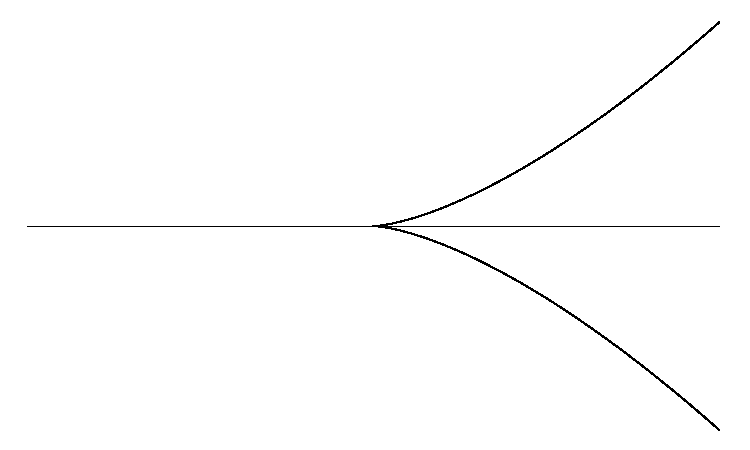
\includegraphics[width=.5\textwidth]{img/cuspidal.pdf}
\caption{a node with some `approximating' lines}
\end{figure}
\paragraph{Case 2: $g=h^2$}
We call the singularity a \emph{cusp}.
Here the image is: The two distinct lines from before collapse to a single double line.
\begin{figure}
\center
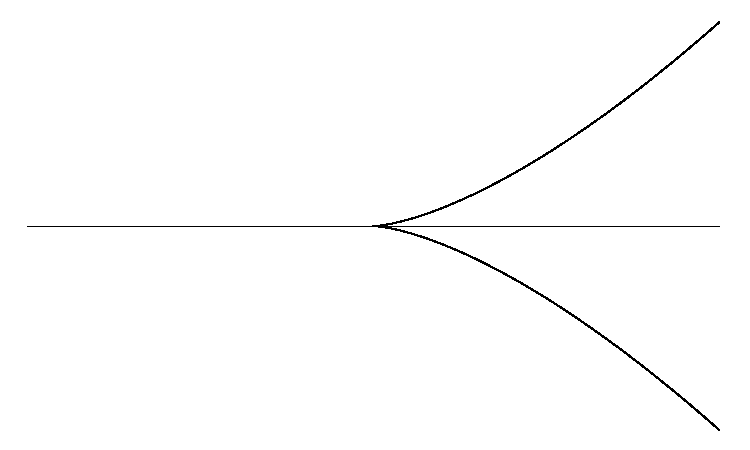
\includegraphics[width=.5\textwidth]{img/nodal.pdf}
\caption{a node with some `approximating' lines}
\end{figure}

Let's summarize the result of this discussion.

\begin{proposition} \label{propositionClassificationOfSingularCubics}
Any irreducible singular cubic curve has precisely one singular of either nodal or cuspidal type.
\end{proposition}


\subsubsection{normal forms of singular cubic curves}

The following discussion on normal forms will follow the argument in \cite[Satz 4.9, p.102]{hulek2000elementare}.
We will obtain in characteristic $\neq 2$ a normal form for cubic curves with nodes and in characteristic $\neq 3$ a normal form for cubic curves with cusps.

First write the cubic $F$ as linear combination of monomials $x^3,xy^2,..z^3$.
As $F$ vanishes at $[0:0:1]$ there is no $z^3$ term.
Likewise there are no $xz^2$ or $yz^2$ terms, because the curve is singular at $[0:0:1]$.
So far $F$ is of the form $zg(x,y) + bx^3 + cx^2y + dxy^2 + ey^3$ where $g$ is some quadratic form.
In fact, $g$ consists of the degree 2 terms of the homogenisation $F(x,y,1$), so it is the same as the quadratic form $g$ in the previous section.

Consider the \emph{nodal case}, i.e. $g=h_1h_2$ where $h_1,h_2$ are $k$-linearly indepent.
This means that we may change the coordinates to $x':=h_1, y':=h_2, z':=z$ (notational convention: this means from now on, for the duration of this derivation of the normal form for nodal cubics, if we write $x$ we mean $h_1$, etc.) and get $F = xyz + b'x^3 + c'x^2y + d'xy^2 + e'y^3$.
Note that neiner $b'$ nor $e'$ may vanish, otherwise we may factor out $x$ or $y$ and we assumed $F$ to be irreducible.
Denote with $\beta$ and $\gamma$ the third roots of $b'$ and $e'$ respectively.
Again we perform another change of coordinates
\begin{equation}
\begin{pmatrix} x' \\ y' \\ z' \end{pmatrix}
:=
\begin{pmatrix}
-\beta^{-1} & -\beta^{-1} & 0 \\
-\gamma^{-1} & \gamma^{-1} & 0 \\
-6\beta\gamma + c'/\beta + d'/\gamma & c'/\beta - d'/\gamma & \beta\gamma
\end{pmatrix}
\begin{pmatrix} x \\ y \\ z \end{pmatrix}
\end{equation}
The matrix has determinant -2, hence this is indeed a base change in characteristic not 2.
After this base change, $F$ has the form $x^2z - y^2z +8x^3$.
A final touch: Set $x' := 2x, y':= 2y,z':=z/4$ to obtain
\begin{proposition} \label{propositionNormalformNodal}
If the characteristic of the ground field is not 2, then every nodal cubic is of the form
\begin{equation}
F = x^2z - y^2z +x^3
\end{equation}
after an appropriate change of coordinates.
\end{proposition}

We turn to the \emph{cuspidal case}, $g = h^2$.
Our first change of coordinates is $y' := h, z' := z$ and let $x' \in k[x,y]$ be any other linear form not in $\var{span}_k(y')$.
This gives us $F = y^2z + b'x^3 + c'x^2y + d'xy^2 + e'y^3$.
Here we can say that $b' \neq 0$, otherwise we may factor out $y'$.
In characteristic not 3 the change of coordinates $x' := x - \frac{c'}{3b'}y$ makes sense.
This eliminates the $x^2y$ term and yields $F = y^2z + b'x^3 +  d''xy^2 + e''y^3$.
Next set $z' := -b'z -d''x -e''y$ to cancel more term: $F = b'(x^3 - y^2z)$.
Finally let $\beta$ be a third root of $b$ and set $x' := \beta x, y' := \beta y, z' := \beta z$:
\begin{proposition} \label{propositionNormalformCuspidal}
If the characteristic of the ground field is not 3, then every cuspidal cubic is of the form
\begin{equation}
F = x^3 - y^2z
\end{equation}
after an appropriate change of coordinates.
\end{proposition}

There is an alternative normal form for the nodal cubic.

\begin{proposition} \label{propositionNormalformNodal2}
If the characteristic of the ground field is not 2, then every nodal cubic is of the form
\begin{equation}
F = x^3 + y^3 + xyz
\end{equation}
after an appropritate change of coordinates.
\end{proposition}

\begin{proof}
We start from the normal form of proposition \ref{propositionNormalformNodal} and perform a change of coordinates
\begin{equation}
\begin{pmatrix} x' \\ y' \\ z' \end{pmatrix}
:=
\frac 12
\begin{pmatrix}
-1 & 1 & 0 \\
-1 & -1 & 0 \\
6 & 0 & 8
\end{pmatrix}
\begin{pmatrix} x \\ y \\ z \end{pmatrix}
\end{equation}
The matrix has determinant $8 \in k^\times$.
\end{proof}
